\documentclass[12pt]{article}
\usepackage[utf8]{inputenc}
\usepackage{parskip}

\usepackage[bottom]{footmisc}
\usepackage{titlesec}

\usepackage[utf8]{inputenc}

\usepackage{graphicx}
\usepackage{subcaption}
\usepackage{wrapfig}

\usepackage{mathtools}
\def\is{\coloneqq}

\usepackage{algorithm,algorithmicx}
\usepackage[noend]{algpseudocode}

\usepackage{caratula}

\begin{document}

\thispagestyle{empty}
\materia{Algoritmos y Estructuras de Datos III}
\submateria{Primer Cuatrimestre de 2019}
\titulo{Trabajo Práctico II}
\subtitulo{Modelando problemas con grafos}
\integrante{Ignacio Losiggio}{751/17}{iglosiggio@dc.uba.ar}
\integrante{Federico Sabatini}{579/17}{sabatinifedericoagustin@gmail.com}

\maketitle
\newpage

\thispagestyle{empty}
\vspace{3cm}
\tableofcontents

\vspace{3cm}

\section{Segmentation is my fault}
\subsection{Introducción y presentación del trabajo realizado}

La segmentación de imágenes de forma es un problema abierto en el área de
\emph{visión artificial} que dada la variedad de sus aplicaciones posee varios
intereses en conflicto al querer desarrollar un algoritmo definitivo para ésta.
Un algoritmo eficiente que requiera tiempo y memoria lineal puede ser útil para
procesamiento de video en tiempo real sacrificando la calida del resultado,
mientras que otro enfoque más costoso puede ser útil a la hora de ofrecer una
herramienta que facilite labores artísticos (separación automática de los
objetos en una escena, por ejemplo).

\begin{figure}[h]
	\centering
	\begin{subfigure}{0.4\linewidth}
		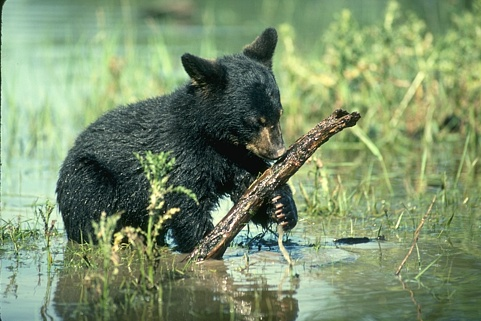
\includegraphics[width=\linewidth]{segmentation/entradas-posta/oso}
		\caption{Entrada}
	\end{subfigure}
	\begin{subfigure}{0.4\linewidth}
		\includegraphics[width=\linewidth]{segmentation/salidas/{0.8.oso.jpg.600.100}.png}
		\caption{Segmentación}
	\end{subfigure}
	\caption{$\sigma = 0.8,\ k = 600,\ g = 100$.}
\end{figure}

El algoritmo a implementar es el propuesto por \textbf{Pedro F.  Felzenszwalb}
y \textbf{Daniel P. Huttenlocher} en su trabajo \textsc{Efficient Graph-Based
Image Segmentation}. Éste algoritmo construye un grafo grilla con cada píxel en
su propio segmento y luego uno los segmentos golosamente dada una condición de
``similaridad suficente'' entre ellos. Para mejorar los resultados del
algoritmo se implementaron dos pasos de pre y post procesamiento.

El preprocesamiento consiste de un desenfoque gaussiano de dos pasadas. Éste se
implementó dentro del programa entregado luego de notar que desenfocar la
imagen y luego guardarla en el formato de entrada propuesto por la cátedra
resultaba en artefactos indeseables propios del bajo rango de valores de cada
pixel. El sigma de desenfoque puede ser modificando variando el segundo
parámetro pasado al ejecutable.

El postprocesamiento es una segunda pasada por las aristas del grafo forzando
la unión de todos los componentes suficientemente chicos. El significado de
``suficientemente chico'' se puede modificar variando el tercer parámetro
pasado al ejecutable. El parámetro es relativo a la resolución de la imagen a
procesar, un valor de $1$ eliminará todas las componentes que posean menos del
$100\%$ de los píxeles, uno de $10$ todas las que posean menos del $10\%$.
Llamaremos $g$ a este parámetro dado que cuanto mayor es su valor mayor es la
\emph{granularidad} de la segmentación resultante\footnote{Efectivamente el
parámetro pone un límite superior a la cantidad de segmentos que puede tener la
segmentación.}.

El algoritmo en sí posee un valor $k$ que representa la ``soltura'' a la hora
de comparar componentes para decidir si unirlas o no. Éste parámetro es el
primero que recibe el ejecutable entregado.

La elección de colores para las segmentaciones mostradas en este informe se
realizó aprovechándose de detalles implementativos. Esta elección nos permite
que los colores sean estables al variar tanto $k$ cómo $g$, lo cuál permitió
crear los videos adjuntos a este informe.

\subsection{Presentación informal e intuitiva del algoritmo}

El algoritmo implementado construye un \emph{grafo grilla} a partir de la
imagen proporcionada y luego recorre las aristas del mismo de menor a mayor
uniendo las compomentes de cada lado de la arista. La motivación es simple,
procesar los píxeles más similares al principio nos forzará a recorrer las
regiones de la imagen desde las de menos variabilidad hasta las que sean
básicamente ruido blanco.

Para tomar la decisión de si unir o no dos componentes se propone calcular la
\emph{diferencia interna} de una componente de la siguiente forma:

\[Int(C) = \max_{a \in AGM(C_V, C_E)} p(a)\]

Dónde $AGM(V, E)$ es el árbol generador mínimo del subgrafo de la componente
$C$, $C_V$ son los vértices de la componente V, $C_E$ son los ejes de la
componente $C$ y $p(e)$ es la función que determina el peso de una
arista\footnote{Dependiendo el espacio de color de la imagen y la forma en la
que se representen los mismos puede haber muchas funciones que tenga sentido
evaluar como $p$.}.

\begin{figure}[h]
	\centering
	\includegraphics[width=0.9\linewidth]{graficos/grilla}
	\caption{Grafo grilla con 8-vecindad.}
\end{figure}

Dado todo esto, dos componentes que limiten en un par de píxeles se unirán si
la diferencia en el límite está dentro de la tolerancia común de las mismas, es
decir si $\textit{diff} \geq Int(C_1) + \tau(C_1) \land \textit{diff} \geq
Int(C_2) + \tau(C_2)$, dónde $\tau(C)$ es la función que le da juego\footnote{\
En el sentido de que suma cierta holgura que permite unir componentes de que
otro parecerían demasiado distintas, cosa que es común con componentes
pequeñas} a la componente. La función propuesta para $\tau(C)$ es la siguiente:

\[\tau(C) = \frac{K}{|C_V|}\]

La que nos ofrece un valor cercano a $K$ para compontentes muy chicas y uno
cercano a $0$ para componentes muy grandes. Ésto fuerza a tener evidencias
claras de que dos componentes son en realidad la misma al ser estas muy grandes
pero nos permite un montón de juego en las primeras etapas.

\subsubsection{Entonces. ¿Cuál es el algoritmo aquí propuesto?}

Construiremos una primera aproximación burda (ubicando cada píxel en su propia
componente) y lo refinaremos preguntándonos si dado un par de componentes
unidas por un eje éstas no deberían en realidad unirse. A la hora de ejecutar
un algorimo así de goloso es importante el orden en el cuál se toman las
aristas a procesar. El obvio (y el utilizado por nosotros) es de menor a mayor
peso\footnote{En una implementación que requiera un tiempo de procesamiento
lineal se puede utilizar un \emph{Counting Sort} sabiendo cuál es la mayor
diferencia posible (256 en el caso de la entrada de la cátedra).}.

Entonces, sumando todos los procesos antes mencionados podemos construir una
suerte de vista aérea de nuestro algoritmo (que nos será útil para luego
ahondar en la implementación de cada parte).

\begin{enumerate}
	\item Cargar la entrada
	\item \textbf{Opcional:} Realizar un desenfoque para evitar
	      ciertos defectos.
	\item Construir el grafo grilla de la entrada, usando la diferencia
	      de intensidades entre píxeles vecinos como peso de cada arista.
	\item Ordenar las aristas construídas por peso.
	\item Construir la solución inicial, asignando a cada píxel (vértice
	      del grafo) en supropia componente.
	\item Por cada arista (de menor a mayor) determinar si los píxeles que
	      une deberían pertenecer a la misma componente. Si es así unirlos.
	\item \textbf{Opcional:} Por cada arista (de menor a mayor) si alguna
	      de las componentes que une es menor al $\frac{100}{g}\%$ de la
	      imagen entonces unir éstas.
	\item Imprimir la salida en el formato deseado, construir colores de
	      ser necesario, etc.
\end{enumerate}

\subsection{El algoritmo (y sus partes)}

En esta sección mostraremos el pseudocódigo correspondiente a este trabajo en
conjunto con información sobre detalles implementativos.

Los algoritmos acá mostrados usan todos alguna implementación de la estructura
\textsc{Disjoint-Set} que posee los siguientes observadores y operaciones:

\begin{itemize}
	\item \Call{Nuevo}{$s$}
		--- Retorna un nuevo \textsc{Disjoint-Set} con $s$ elementos.
	\item \Call{Buscar}{ds, $e$}
		--- Retorna el identificador de la componente de $e$.
	\item \Call{Unir}{ds, $a$, $b$}
		--- Une al componente que contiene a $a$ con el componente que
		contiene a $b$.
	\item \Call{Tamaño}{ds, $e$}
		--- Retorna el tamaño (en cantidad de elementos) de la
		componente que contiene a $e$.
\end{itemize}

\subsubsection{Desenfoque}

La implementación del desenfoque depende se realiza generando el \emph{kernel}
con el $\sigma$ apropiado. Y aprovecharnos de la \emph{separabilidad} del
filtro para hacer una convolución en cada eje en lugar de tener que usar la
matriz completa. Por otro lado elegimos limitar la cantidad de términos de la
máscara a los que naturales desde $0$ hasta $\lceil 4 \sigma \rceil$ cuando
necesitamos valores negativos de la normal los reflejamos en el \emph{kernel}
calculado. El tope que escojemos hace que los coeficientes fuera del
\emph{kernel} sean menores a $e^{-8}$ que son suficentemente pequeños cómo para
no resultarnos relevantes.

\begin{algorithm}[H]
\caption{Algoritmo para realizar un desenfoque gaussiano}
\begin{algorithmic}[1]
\Statex{}
\Function{Desenfocar}{$w$, $h$, imagen, $\sigma$}`
	\Statex{} \Comment{} Por simpleza no están los chequeos de límites en la imagen
	\State{} $\text{kernel} \is []$
	\For{$i \is 0$ to $\lceil 4 \sigma \rceil + 1$}
	\Comment{Coefficientes de la normal a usar}
		\State{} $\text{kernel}[i]
			\is \frac{1}{\sqrt{2\pi\sigma^2}}e^{-\frac{i^2}{2\sigma^2}}$
	\EndFor{}
	\For{$y \is 0$ to $h$}
		\Comment{} Convolución horizontal
		\For{$x \is 0$ to $w$}
			\State{} $\text{sum} \is 0$
			\For{$i \is 0$ to $|\text{kernel}|$}
				\State{} $\text{sum} \is \text{sum}
					+ \text{kernel}[i] \times (
						\text{imagen}[y][x - 1]
						+ \text{imagen}[y][x + 1]
					)$
			\EndFor{}
			\State{} $\text{imagen}[y][x] \is \text{sum}$
		\EndFor{}
	\EndFor{}
	\For{$y \is 0$ to $h$}
		\Comment{} Convolución vertical
		\For{$x \is 0$ to $w$}
			\State{} $\text{sum} \is 0$
			\For{$i \is 0$ to $|\text{kernel}|$}
				\State{} $\text{sum} \is \text{sum}
					+ \text{kernel}[i] \times (
						\text{imagen}[y - 1][x]
						+ \text{imagen}[y + 1][x]
					)$
			\EndFor{}
			\State{} $\text{imagen}[y][x] \is \text{sum}$
		\EndFor{}
	\EndFor{}
\EndFunction{}
\end{algorithmic}
\end{algorithm}

\subsubsection{Construcción del grafo}

Para construir el grafo utilizamos la 8-vecindad cómo ya dijimos anteriormente.
Una vez cargada la imagen podemos recorrer todos los píxeles (que serán
vértices de nuestro grafo) y agregar los ejes necesarios.

\begin{algorithm}[H]
\caption{Algoritmo para construir el grafo a segmentar}
\begin{algorithmic}[1]
\Statex{}
\Function{Construir-Grafo}{$w$, $h$, imagen}
	\Statex{} \Comment{} Describimos a los ejes como \{desde, hasta, peso\}
	\State{} $\text{ejes} \is \emptyset$
	\For{$y \is 0$ to $h$}
		\For{$x \is 0$ to $w$}
			\State{} $p_o \is \{x, y\}$
			\State{} $p_e \is \{x + 1, y\}$
			\If{$p_e$ está en los límites de la imagen}
				\State{} $\text{dif}
					\is \Call{Diferencia}{p_o,\ p_e,\ \text{imagen}}$
				\State{} \Call{Agregar}{ejes, \{$p_o$, $p_e$, dif\}}
			\EndIf{}
			\State{} $p_{sw} \is \{x - 1, y + 1\}$
			\If{$p_{sw}$ está en los límites de la imagen}
				\State{} $\text{dif}
					\is \Call{Diferencia}{p_o,\ p_{sw},\ \text{imagen}}$
				\State{} \Call{Agregar}{ejes, \{$p_o$, $p_{sw}$, dif\}}
			\EndIf{}
			\State{} $p_s \is \{x, y + 1\}$
			\If{$p_s$ está en los límites de la imagen}
				\State{} $\text{dif}
					\is \Call{Diferencia}{p_o,\ p_s,\ \text{imagen}}$
				\State{} \Call{Agregar}{ejes, \{$p_o$, $p_s$, dif\}}
			\EndIf{}
			\State{} $p_{se} \is \{x + 1, y + 1\}$
			\If{$p_{se}$ está en los límites de la imagen}
				\State{} $\text{dif}
					\is \Call{Diferencia}{p_o,\ p_{se},\ \text{imagen}}$
				\State{} \Call{Agregar}{ejes, \{$p_o$, $p_{se}$, dif\}}
			\EndIf{}
		\EndFor{}
	\EndFor{}
	\State{} \Return{} ejes
\EndFunction{}
\end{algorithmic}
\end{algorithm}

\subsubsection{Segmentación}

Con los ejes ya ordenados el proceso de segmentar la imagen es muy simple.
$\tau(C)$ es la función que dado un identificador de componente indica el
factor de juego que le corresponde a esa componente.

\begin{algorithm}[H]
\caption{Algoritmo segmentar el grafo generado}
\begin{algorithmic}[1]
\Statex{}
\Function{Segmentar}{$w$, $h$, ejes}
	\State{} $\text{ds} \is \Call{Nuevo}{w \times h}$
	\State{} $\text{umbral} \is [\tau(0), \tau(1), \dots, \tau(w \times h - 1)]$
	\For{$\text{eje} \in \text{grafo}$ (de menor a mayor peso)}
		\State{} $C_a \is \Call{Buscar}{\text{ds},\ \text{eje}.\text{desde}}$
		\State{} $C_b \is \Call{Buscar}{\text{ds}\, \text{eje}.\text{hasta}}$
		\If{$\text{eje}.\text{peso} \leq \text{umbral}[C_a]
			\land \text{eje}.\text{peso} \leq \text{umbral}[C_b]$}
			\State{} \Call{Unir}{ds, $C_a$, $C_b$}
			\State{} $C_a \is \Call{Buscar}{\text{ds},\ C_a}$
			\State{} $\text{umbral}[C_a] \is \Call{Tamaño}{\text{ds},\ C_a}
				+ \tau(C_a)$
		\EndIf{}
	\EndFor{}
	\State{} \Return{} ds
\EndFunction{}
\end{algorithmic}
\end{algorithm}

\subsubsection{Simplificación Greedy}

Una vez segmentada la imagen se puede realizar un paso final que elimine las
componentes más pequeñas. El recorrer las aristas de menor a mayor peso hace
que las componentes que se unifiquen siempre lo hagan por la arista más liviana
de su frontera (que es lógico suponer pertenece a la componente limítrofe más
parecida).

\begin{algorithm}[H]
\caption{Algoritmo para eliminar segmentos pequeños}
\begin{algorithmic}[1]
\Statex{}
\Function{Simplificar}{$w$, $h$, ds, ejes, $g$}
	\State{} $\text{min} \is \frac{g}{w \times h}$
	\For{$\text{eje} \in \text{ejes}$ (de menor a mayor peso)}
		\If{$\Call{Tamaño}{\text{ds, eje}_a} < \text{min}
		     \vee \Call{Tamaño}{\text{ds, eje}_b} < \text{min}$}
			\State{} $C_a \is \Call{Buscar}{\text{ds, eje}_a}$
			\State{} $C_b \is \Call{Buscar}{\text{ds, eje}_b}$
			\If{$C_a \neq C_b$}
				\State{} \Call{Unir}{ds, $C_a$, $C_b$}
			\EndIf{}
		\EndIf{}
	\EndFor{}
\EndFunction{}
\end{algorithmic}
\end{algorithm}

\subsubsection{Vista aérea del algoritmo}

A modo de unificar todos los pasos ya expuestos en detalle podemos resumir la
operación del algoritmo en pocas líneas:

\begin{algorithm}[H]
\caption{Algoritmo para segmentar con todos los pasos comentados}
\begin{algorithmic}[1]
\Statex{}
\Function{Simplificar}{$w$, $h$, imagen, $\sigma$, $k$, $g$}
	\State{} \Call{Desenfocar}{$w$, $h$, imagen, $\sigma$}
	\State{} $\text{ejes} \is \Call{Construir-Grafo}{w,\ h,\ \text{imagen}}$
	\State{} \Call{Ordenar}{ejes}
	\State{} $\text{segmentación} \is \Call{Segmentar}{w,\ w,\ \text{ejes}}$
	\State{} \Call{Simplificar}{$w$, $h$, segmentación, ejes, $g$}
	\State{} \Return{} segmentacion
\EndFunction{}
\end{algorithmic}
\end{algorithm}

\subsection{Estructuras para implementar \textsc{Disjoint-Set}}

Como parte del trabajo la cátedra requirió implementar el \textsc{Disjoint-Set}
con 3 estructuras distintas, las listamos en conjunto con la complejidad de las
operaciones antes descriptas:

\begin{itemize}
	\item Representado como arreglo de componentes
	\begin{itemize}
		\item \Call{Nuevo}{s}: $O(s)$
		\item \Call{Buscar}{ds, $e$}: $O(1)$
		\item \Call{Unir}{ds, $a$, $b$}: $O(n)$
		\item \Call{Tamaño}{ds, $e$}: $O(1)$
	\end{itemize}
	\item Representado como árbol
	\begin{itemize}
		\item \Call{Nuevo}{s}: $O(s)$
		\item \Call{Buscar}{ds, $e$}: $O(n)$
		\item \Call{Unir}{ds, $a$, $b$}: $O(1)$
		\item \Call{Tamaño}{ds, $e$}: $O(1)$
	\end{itemize}
	\item Representado como árbol con \emph{path compression}
	\begin{itemize}
		\item \Call{Nuevo}{s}: $O(s)$
		\item \Call{Buscar}{ds, $e$}: $O(\alpha(s))$
			\textbf{(amortizado)}
		\item \Call{Unir}{ds, $a$, $b$}: $O(\alpha(s))$
			\textbf{(amortizado)}
		\item \Call{Tamaño}{ds, $e$}: $O(\alpha(s))$
			\textbf{(amortizado)}
	\end{itemize}
\end{itemize}

Sumado a esto, las representaciones de árbol pueden elegir si unir por mayor
rango o por mayor tamaño (en nuestro caso particular implementamos por mayor
tamaño).

\subsubsection{Resultados con distintos tamaños de imagen}

En este apartado buscamos determinar el comportamiento de nuestras
implementaciones dados diferentes tamaños de imagen. Queremos verificar en cada
uno de ellos como varía el timpo de ejecución. 

Usaremos 3 imagenes con dimensiones cuadradas por su facilidad para
redimensionarlas. Las resoluciones a utilizar serán $[100 \times
100\text{px},200 \times 200\text{px}, \dots, 700 \times 700\text{px}]$.

\begin{figure}[H]
	\centering
	\begin{subfigure}{0.3\linewidth}
		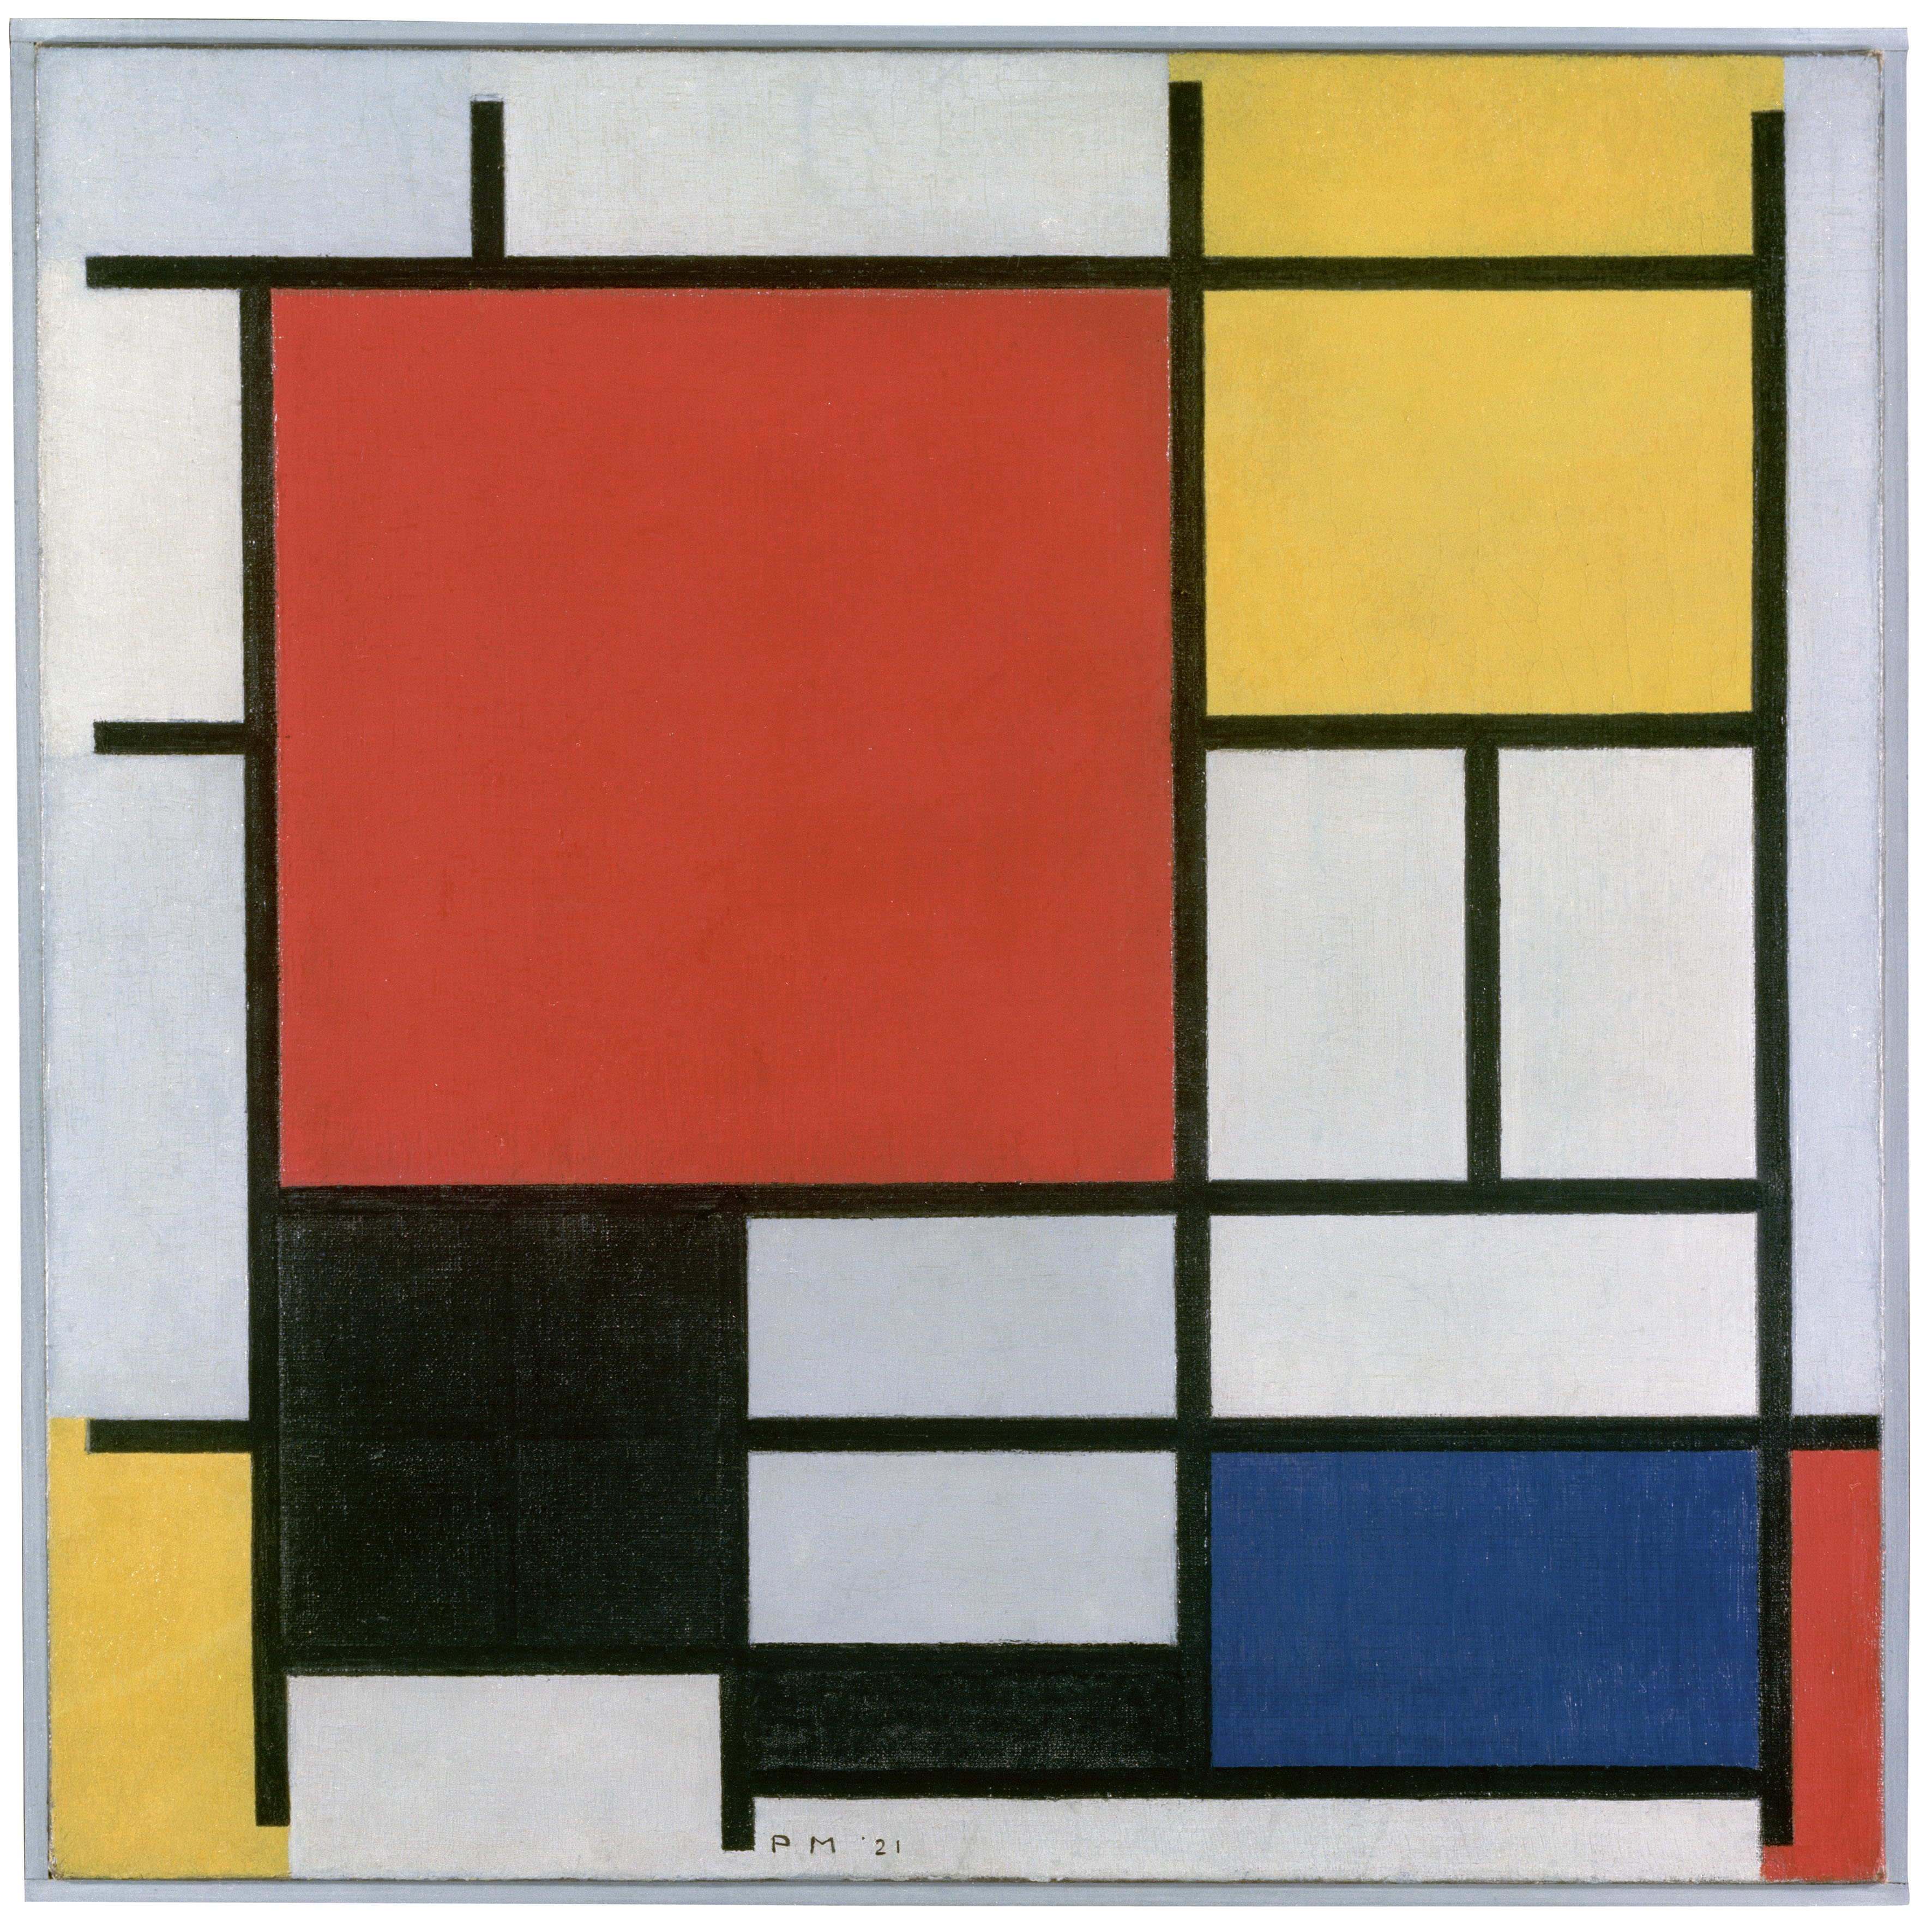
\includegraphics[width=\linewidth]{segmentation/entradas-posta/mondrian}
		\caption{\texttt{mondrian.jpg}}
	\end{subfigure}
	\begin{subfigure}{0.3\linewidth}
		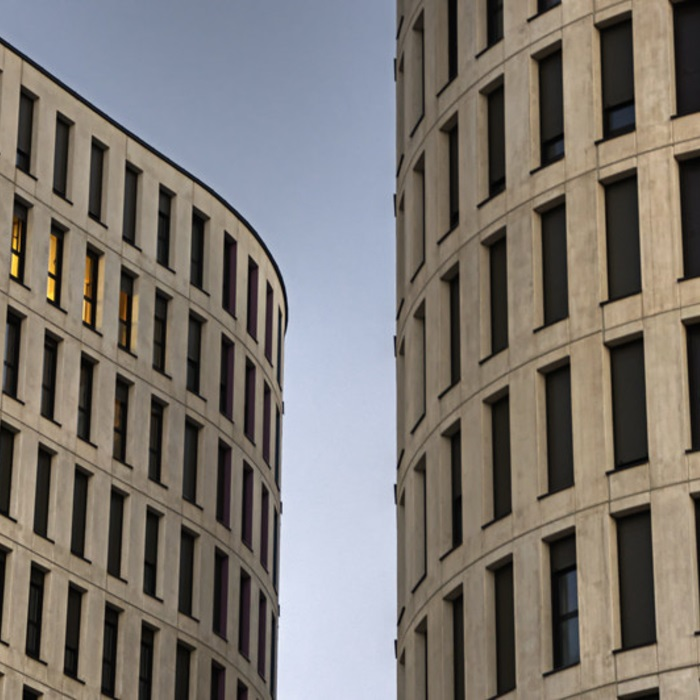
\includegraphics[width=\linewidth]{segmentation/entradas-posta/edificios}
		\caption{\texttt{edificios.png}}
	\end{subfigure}
	\begin{subfigure}{0.3\linewidth}
		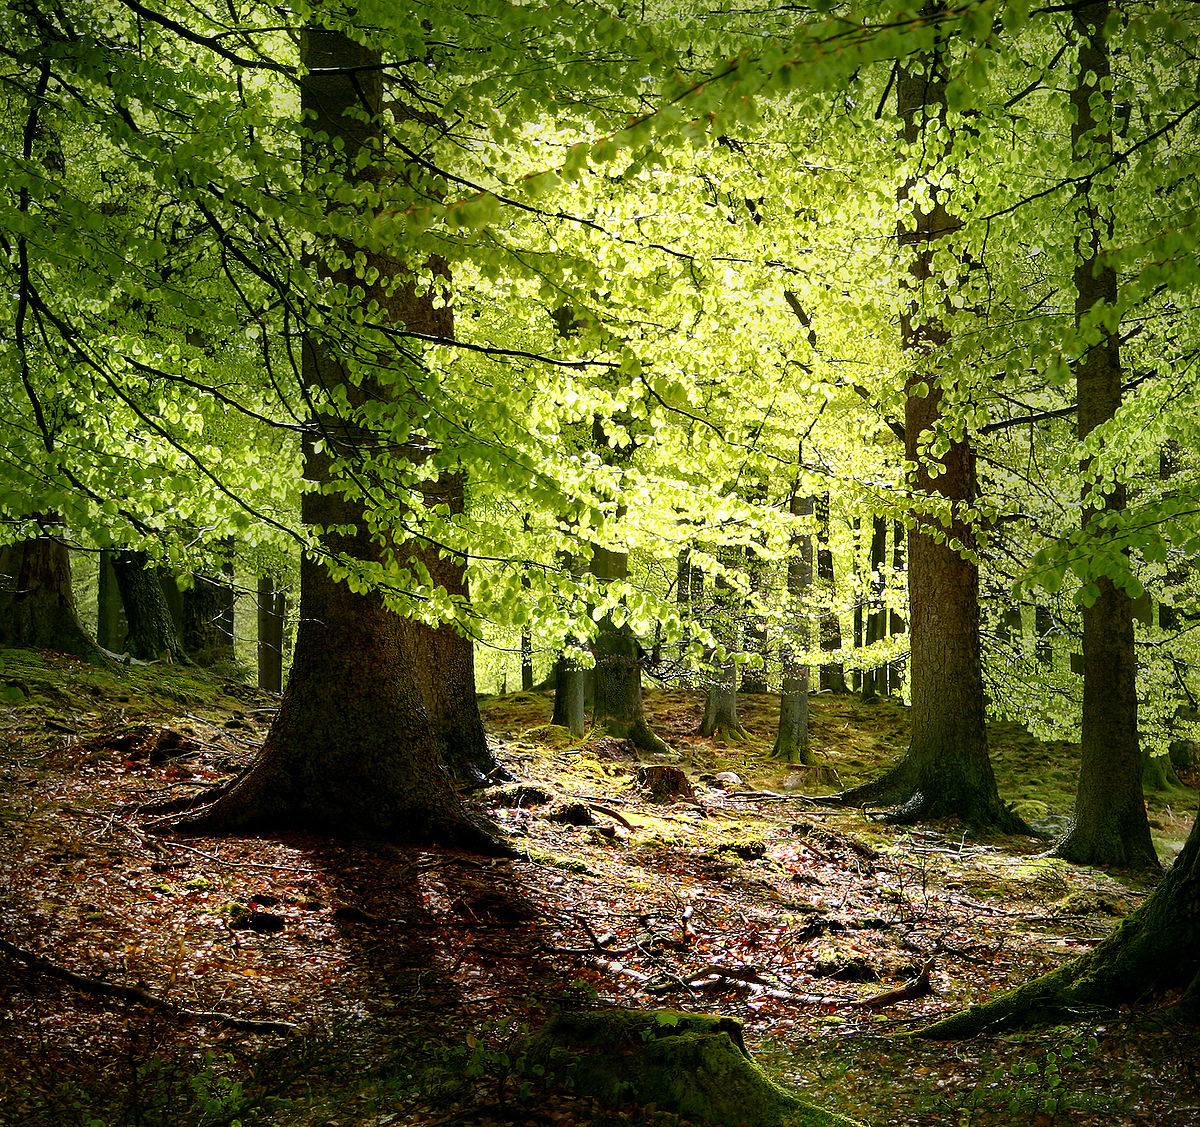
\includegraphics[width=\linewidth]{segmentation/entradas-posta/bosque}
		\caption{\texttt{bosque.jpg}}
	\end{subfigure}
\end{figure}

Las 3 imágenes han sido seleccionadas para probar tres casos claros: (a)
posee varias regiones planas sobre las cuales el algoritmos ejecutará
\textsc{Union} muchas veces, (b) tiene una textura dominante que al no ser
del todo plana generará varios segmentos de pocos píxeles y (c) tiene muchos
pequeños detalles que harán que se generen montones de segmentos.

Los parámetros para cada corrida serán $k = 300$, $\sigma = 0.8$ sin paso de
simplificación. Para ver el efecto que tiene variar los parámetros en el tiempo
de ejecución tendremos una sección más adelante.

\begin{figure}[H]
	\centering
	\includegraphics[width=0.75\linewidth]{segmentation/experimentacion/distintas-fotos-arreglo}
	\caption{Segmentación implementando \textsc{Disjoint-Set} con arreglo.}
\end{figure}

\begin{figure}[H]
	\centering
	\includegraphics[width=0.75\linewidth]{segmentation/experimentacion/distintas-fotos-arbol}
	\caption{Segmentación implementando \textsc{Disjoint-Set} con un árbol.}
\end{figure}

\begin{figure}[H]
	\centering
	\includegraphics[width=0.75\linewidth]{segmentation/experimentacion/distintas-fotos-arbol-compr}
	\caption{Segmentación implementando \textsc{Disjoint-Set} con un árbol con compresión.}
\end{figure}

En los 3 algoritmos podemos observar un comportamiento similar, siendo el
algoritmo de árbol de compresión el que muestra un rendimiento superior
(alrededor de dos veces más rápido que el resto). Esto no se condice con la
complejidad teórica, pero puede deberse a que el eje X de los gráficos no
representa un cambio lineal en el tamaño de la entrada.

Otra cosa notable es que pese a las claras diferencias entre las imágenes todos
los algoritmos tienen un comportamiento similar dada una misma resolución de
imagen.

\subsubsection{Influencia de los parámetros}

Esta sección del informe analiza el rendimiento de las distintas
representaciones variando los parámetros $k$ y $g$\footnote{Valores de $\sigma$
mayores aumentarían el tiempo requerido de procesamiento pero ese procesamiento
se realiza antes de cualquier llamada a las estructuras que son relevantes a
esta sección del informe.}.

Dado que \textsc{Buscar} es considerablemente más simple en las
implementaciones con arreglo de componententes creemos que es esperable que
presente un rendimiento levemente superior para valores de $k$ y $g$ muy bajos
(dónde se realizan muy pocas llamadas a \textsc{Unir}).

Para realizar estos experimentos tomamos una sola imagen como entrada
(\texttt{autitos.jpg}) sobre la cuál experimentamos. La decisión de tomar una
única imagen fué debido a que queremos medir el efecto de los parámetros en una
imagen dónde estos tengan relevancia (en una imagen completamente plana variar
$k$ o $g$ no cambiaría la segmentación resultante, las llamadas a \textsc{Unir}
y \textsc{Buscar} serían siempre las mismas).

\begin{figure}[h]
	\centering
	\begin{subfigure}{0.4\linewidth}
		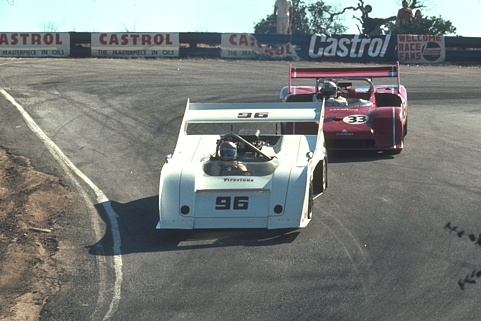
\includegraphics[width=\linewidth]{segmentation/entradas-posta/autitos}
		\caption{Entrada}
	\end{subfigure}
	\begin{subfigure}{0.4\linewidth}
		\includegraphics[width=\linewidth]{segmentation/salidas/{0.8.autitos.jpg.300.1000}.png}
		\caption{Segmentación}
	\end{subfigure}
	\caption{$\sigma = 0.8,\ k = 300,\ g = 1000$.}
\end{figure}

\subsubsection{Resultados variando $k$}

En el primer experimento decidimos medir el tiempo que tardaba el paso de
segmentación variando el $k$ de $0$ a $1200$ con incrementos de a $50$.

\begin{figure}[h]
	\centering
	\includegraphics[width=0.75\linewidth]{segmentation/experimentacion/variar-k}
	\caption{Tiempo incurrido por el proceso de segmentar al variar el $k$}
\end{figure}

Cuándo $k$ es $0$ el gráfico muestra que la segmentación realiza poco trabajo,
pero a partir de $50$ no muestra ninguna tendencia clara. Cómo la
experimentación se realizó con la misma entrada siempre esto da indicios de que
el coste de este trabajo no se ve influído más que por las características del
grafo grilla que se construye.

\subsubsection{Resultados variando $g$}

Dado que la granularidad varía su trabajo de acuerdo al $k$ elegido decidimos
tomar $k$ entre $0$ y $1200$ y variar el $g$ entre $1$ y $991$ en incrementos
de $10$.

\begin{figure}[h]
	\centering
	\includegraphics[width=0.75\linewidth]{segmentation/experimentacion/variar-g-arreglo}
	\caption{Tiempo incurrido por el proceso de simplificar al variar el $g$}
\end{figure}

Para $k=0$ vemos que cómo que el set resultante de la segmentación tenga
muchísimos conjuntos pequeños logra que el tiempo que requiera la
simplificación sea considerablemente mayor. También vemos que cada
implementación llega a un mínimo dado un $g$ suficientemente alto dónde el
costo de hacer las llamadas a \textsc{Tamaño} superan a las pocas llamadas a
\textsc{Unir} resultantes de los chequeos.

\begin{figure}[h]
	\centering
	\includegraphics[width=0.75\linewidth]{segmentation/experimentacion/variar-g-arbol}
	\caption{Tiempo incurrido por el proceso de simplificar al variar el $g$}
\end{figure}

Tomar el árbol como representación el caso de $k=0$ arroja resultados
interesantes. Dado que no se comprime el árbol cuanto menos se unifiquen las
componentes menor es el coste de \textsc{Tamaño} que internamente realiza una
llamada a \textsc{Buscar}. Lamentablemente cómo no experimentamos con mayor
finura en los valores de $k$ entre $1$ y $150$ no podemos decir nada sobre cuál
sea la tendencia que toma el gráfico en ese rango, sí vemos una tendencia más
clara para el resto de los valores que tenemos información.

\clearpage

\begin{figure}[h]
	\centering
	\includegraphics[width=0.75\linewidth]{segmentation/experimentacion/variar-g-arbol-compr}
	\caption{Tiempo incurrido por el proceso de simplificar al variar el $g$}
\end{figure}

Finalmente, en la simplificación usando la representación de árbol con
compresión volvemos a ver las tendencias de la representación de arreglo pero
con tiempos la mitad de grandes. Dado que los costes teóricos deberían ser
diferentes pero vemos tendencias muy similares esto nos da indicios de que
nuestro experimento no supo elegir valores que evidencien esas
diferencias\footnote{O que nuestras implementaciones tienen errores que hacen
que no funcionen de la forma esperada.}

\clearpage

\subsection{Análisis de resultados}

Sumado a la comparación entre distintas implementaciones del
\textsc{Disjoint-Set} en esta sección mostraremos segmentaciones resultantes de
ejecutar el algoritmo con distintos parámetros. También se ofrecen adjuntos
tres videos dónde se varía cada uno de los parámetros mientras se fijan los
otros dos\footnote{Dado que la forma en la que elegimos los colores no resultó
estable respecto de variar $\sigma$ el video dónde se lo varía podría resultar
molesto para personas con fotosensibildad.}.

\begin{figure}[h]
	\centering
	\begin{subfigure}{0.4\linewidth}
		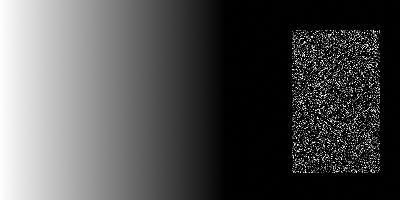
\includegraphics[width=\linewidth]{segmentation/entradas-posta/sintetico}
		\caption{Entrada}
	\end{subfigure}
	\begin{subfigure}{0.4\linewidth}
		\includegraphics[width=\linewidth]{segmentation/salidas/{0.8.sintetico.png.500.1000}.png}
		\caption{Segmentación}
	\end{subfigure}
	\caption{$\sigma = 0.8,\ k = 500,\ g = 1000$.}
\end{figure}

Una buena segmentación es un concepto difícil de definir, dado que depende el
nivel de granularidad deseado ciertos segmentos pueden resultar útiles o no
(ventanas en edificios, ojos en personas, letras individuales en una hoja,
etc). Cómo nuestro algoritmo sólo percibe la intensidad de cada píxel se pierde
información propia del color en la transformación que nos genera casos de error
que podrían salvarse de otro modo.

\subsubsection{Errores esperables}

Escojer un bien el valor de $\sigma$ resulta importante para eliminar ciertas
imperfecciones. Valores de entre $0.4$ t $0.8$ fueron los que utilizamos para
ver los resultados\footnote{Se puede correr \texttt{make ver\_todos} en
\texttt{segmentation} para ver los resultados con $\sigma = 0.8$, $k = 600$ y
sin pasada de simplificación. También se pueden pasar los valores como
parámetro en la forma \texttt{make BLUR=$\sigma$ K=$k$ MIN=$g$ ver\_todos}.}.

En las siguientes imágenes se pueden apreciar distintas segmentaciones de uno
de las imágenes que no pudimos encontrar un conjunto de parámetros que ofrezcan
una segmentación razonable. Dado que la evidente diferencia de color no se
traslada a la entrada en escala de grises. Puede observarse cómo el proceso de
simplificación mantiene algunos de los limites de la imagen original para
valores de $k$ muy bajos y cómo pu puede ser útil eliminar segmentos demasiado
chicos con esa técnica en lugar de elevar el $k$ perdiendo los segmentos del
insecto.

\begin{figure}[h]
	\centering
	\begin{subfigure}{0.4\linewidth}
		
\includegraphics[width=\linewidth]{segmentation/entradas-posta/mariquita}
		\caption{Entrada}
	\end{subfigure}
	\begin{subfigure}{0.4\linewidth}
		
\includegraphics[width=\linewidth]{segmentation/informe/mariquita}
		\caption{Entrada en escala de grises}
	\end{subfigure}
	\begin{subfigure}{0.4\linewidth}
		\includegraphics[width=\linewidth]{segmentation/salidas/{0.0.mariquita.jpg.6000.-1}.png}
		\caption{$\sigma = 0,\ k = 6000$}
	\end{subfigure}
	\begin{subfigure}{0.4\linewidth}
		\includegraphics[width=\linewidth]{segmentation/salidas/{0.0.mariquita.jpg.0.1000}.png}
		\caption{$\sigma = 0,\ k = 0,\ g = 1000$}
	\end{subfigure}
	\begin{subfigure}{0.4\linewidth}
		\includegraphics[width=\linewidth]{segmentation/salidas/{0.0.mariquita.jpg.600.-1}.png}
		\caption{$\sigma = 0,\ k = 600$}
	\end{subfigure}
	\begin{subfigure}{0.4\linewidth}
		\includegraphics[width=\linewidth]{segmentation/salidas/{0.0.mariquita.jpg.600.1000}.png}
		\caption{$\sigma = 0,\ k = 600,\ g = 1000$}
	\end{subfigure}
	\caption{Distintas configuraciones con distintos tipos de error,
	aquellas que no especifican valores para $g$ no tuvieron paso de
	simplificación.}
\end{figure}

\clearpage

La importancia del desenfoque no es evidente en todas las imágenes, la
siguiente escena muestra un defecto que ocurre cuando las fotos tienen mucho
grano:

\begin{figure}[h]
	\centering
	\begin{subfigure}{0.3\linewidth}
		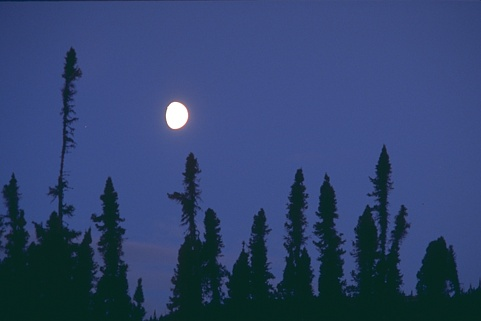
\includegraphics[width=\linewidth]{segmentation/entradas-posta/noche}
		\caption{Entrada}
	\end{subfigure}
	\begin{subfigure}{0.3\linewidth}
		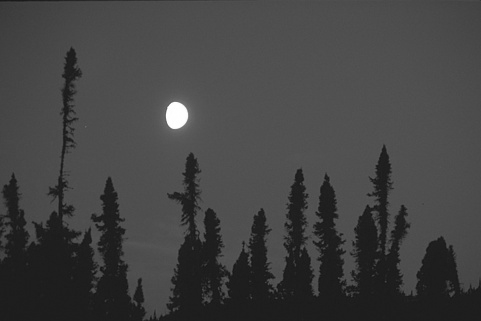
\includegraphics[width=\linewidth]{segmentation/informe/noche}
		\caption{Escala de grises}
	\end{subfigure}
	\begin{subfigure}{0.3\linewidth}
		\includegraphics[width=\linewidth]{segmentation/salidas/{0.0.noche.jpg.600.-1}.png}
		\caption{$\sigma = 0,\ k = 600$}
	\end{subfigure}
	\begin{subfigure}{0.3\linewidth}
		\includegraphics[width=\linewidth]{segmentation/salidas/{0.2.noche.jpg.600.-1}.png}
		\caption{$\sigma = 0.2,\ k = 0$}
	\end{subfigure}
	\begin{subfigure}{0.3\linewidth}
		\includegraphics[width=\linewidth]{segmentation/salidas/{0.4.noche.jpg.600.-1}.png}
		\caption{$\sigma = 0.4,\ k = 600$}
	\end{subfigure}
	\begin{subfigure}{0.3\linewidth}
		\includegraphics[width=\linewidth]{segmentation/salidas/{0.6.noche.jpg.600.-1}.png}
		\caption{$\sigma = 0.6,\ k = 600$}
	\end{subfigure}
	\begin{subfigure}{0.4\linewidth}
		\includegraphics[width=\linewidth]{segmentation/salidas/{0.8.noche.jpg.600.-1}.png}
		\caption{$\sigma = 0.8,\ k = 600$}
	\end{subfigure}
	\begin{subfigure}{0.4\linewidth}
		\includegraphics[width=\linewidth]{segmentation/salidas/{1.0.noche.jpg.600.-1}.png}
		\caption{$\sigma = 1,\ k = 600$}
	\end{subfigure}
	\caption{Segmentación de una escena simple con grano.}
\end{figure}

\clearpage

\subsubsection{Resultados favorables}

\begin{figure}[h]
	\centering
	\begin{subfigure}{0.3\linewidth}
		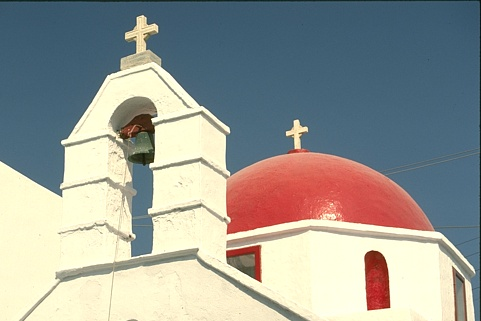
\includegraphics[width=\linewidth]{segmentation/entradas-posta/iglesia}
		\caption{Entrada}
	\end{subfigure}
	\begin{subfigure}{0.3\linewidth}
		\includegraphics[width=\linewidth]{segmentation/salidas/{0.8.iglesia.jpg.600.-1}.png}
		\caption{$\sigma = 0.8,\ k = 600$}
	\end{subfigure}
	\begin{subfigure}{0.3\linewidth}
		\includegraphics[width=\linewidth]{segmentation/salidas/{0.8.iglesia.jpg.600.1000}.png}
		\caption{$g = 1000$}
	\end{subfigure}
	\caption{Segmentacion de \texttt{iglesia.jpg}}
\end{figure}

\begin{figure}[h]
	\centering
	\begin{subfigure}{0.3\linewidth}
		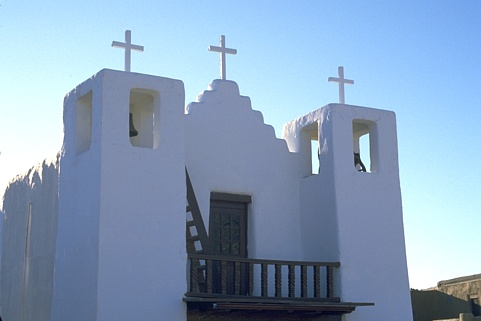
\includegraphics[width=\linewidth]{segmentation/entradas-posta/iglesia_2}
		\caption{Entrada}
	\end{subfigure}
	\begin{subfigure}{0.3\linewidth}
		\includegraphics[width=\linewidth]{segmentation/salidas/{0.8.iglesia_2.jpg.600.-1}.png}
		\caption{$\sigma = 0.8,\ k = 600$}
	\end{subfigure}
	\begin{subfigure}{0.3\linewidth}
		\includegraphics[width=\linewidth]{segmentation/salidas/{0.8.iglesia_2.jpg.600.1000}.png}
		\caption{$g = 1000$}
	\end{subfigure}
	\caption{Segmentacion de \texttt{iglesia\_2.jpg}}
\end{figure}

\begin{figure}[h]
	\centering
	\begin{subfigure}{0.3\linewidth}
		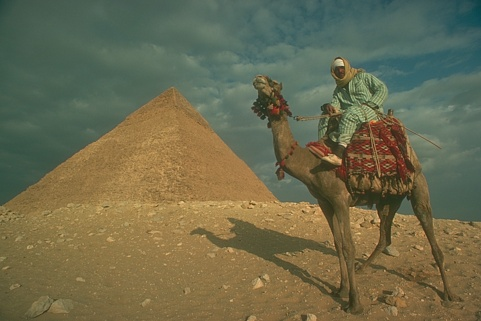
\includegraphics[width=\linewidth]{segmentation/entradas-posta/piramide_camello}
		\caption{Entrada}
	\end{subfigure}
	\begin{subfigure}{0.3\linewidth}
		\includegraphics[width=\linewidth]{segmentation/salidas/{0.8.piramide_camello.jpg.300.-1}.png}
		\caption{$\sigma = 0.8,\ k = 300$}
	\end{subfigure}
	\begin{subfigure}{0.3\linewidth}
		\includegraphics[width=\linewidth]{segmentation/salidas/{0.8.piramide_camello.jpg.300.1000}.png}
		\caption{$g = 1000$}
	\end{subfigure}
	\caption{Segmentacion de \texttt{piramide\_camello.jpg}}
\end{figure}

Cómo puede observarse, dado suficiente contraste el algoritmo genera
segmentaciones razonables, aunque por usar la 8-vecindad de cada píxel
construye pequeños segmentos en lugares quese ven cortados por una sombra.

\subsection{Conclusiones y trabajo futuro}

Con lo expuesto anteriormente está claro que el resultado de esta técnica es
muy sensible a los parámetros dados y a la claridad de la imagen de entrada.
Buscar heurísticas para encontrar éstos es un camino posible para facilitar el
uso del algoritmo así cómo otras formulaciones para la diferencia entre píxeles
y para $\tau(C)$.

Otro punto en el cual creemos que faltó trabajo es en utilizar diferentes
imágenes para ver cómo afectan al tiempo dadas las distintas implementaciones.
de \textsc{Disjoint-Set}. Creemos también que los videos que complementan éste
informe resultan útiles para entender las cualidades de la técnica. Pero dado
que la selección de colores no es estable respecto de $\tau$ una estrategia
mejor para construir las visualizaciones variando los parámetros es algo que
creemos nos faltó.



\section{Llenalo con super}

\subsection{Presentación del problema}
Dado un vendedor que cuenta con vehiculo propio que necesita moverse entre ciudades personalmente para vender sus productos, se quiere buscar la manera más económica de realizar la tarea.

Las distancias entre ciudades están representadas en kilometros y el costo de la nafta también es por kilometro luego se quiere minimizar el costo máximo de llegar de cada ciudad a todas las demás teniendo en cuenta las siguientes propiedades: 

\begin{enumerate}
	\item Las rutas que comunican las ciudades son bidireccionales.
	\item El precio de la nafta varía en cada ciudad.
	\item El auto posee un limite de nafta que puede cargar (máximo para 60 kilometros).
	\item El auto siempre empieza con el tanque vacio.
\end{enumerate}

Puede observarse que el problema es representable con grafos donde las ciudades $c_i$ son los vertices cada una con un costo de nafta $q_i$ asociado. Donde cada distancia $d_{x,y}$ que comunica un par de ciudades $(c_x, c_y)$ sin perdida de generalidad son las $m$ aristas del grafo. 

Además se denominará $l_i \in [0,60]$ como la cantidad de nafta cargada en una ciudad. 

Se representará entonces como un camino posible entre dos ciudades a $P_{k_{x,y}}$ en función del costo total en nafta de realizarlo. Nos interesa los caminos $P_{min_{x,y}}$ que cumplen:

$\forall(c_x, c_y \in Ciudades)(P_{min_{x,y}}, P_{k_{x,y}} \in Caminos(c_x,c_y))\rightarrow(P_{min} < P_k)$

Es decir nos interesan todos los caminos minimos.

Una motivación razonable para resolver el problema sería aplicar algoritmos de grafos conocidos de camino minimo, sin embargo nos encontramos con una serie de inconvenientes.

El costo de cargar nafta en una ciudad se encuentra en función de los vertices, no depende de las distancias, Sino de una multiplicación de $l_i$ por su respectivo precio $q_i$.

Las rutas son bidireccionales, sin embargo dadas 2 ciudades $c_a$ y $c_b$ no se cumple que los costes $c_a \rightarrow c_b$ y $c_b \rightarrow c_a$ sean iguales.

Eso significa que una representación direccional con digrafos podría resultar más adecuada para representar los costes efectivos. En las figuras posteriores se ilustran esta diferencia para 2 ciudades.

\begin{minipage}{0.5\textwidth}
	\includegraphics[width=\linewidth]{{graficos/direccional}.pdf}
	\captionof{figure}{bidireccional}
\end{minipage}
\begin{minipage}{0.5\textwidth}
	\includegraphics[width=\linewidth]{{graficos/bidireccional}.pdf}
	\captionof{figure}{direccional}
\end{minipage}

En particular $\forall(p_a \neq p_b) \rightarrow (p_a * d_{a,b} \neq p_b * d_{a,b}) $

Además los caminos minimos no necesariamente son simples, por ejemplo dadas 3 ciudades $c_a$, $c_b$ y $c_c$ y 2 rutas con distancia $d_{a,b}$ y $d_{a,c}$.

\begin{minipage}{0.5\textwidth}
	Tengo que si $q_a > q_b$ podría tener que evaluar si moverme allí para cargar nafta y volver es menos costoso, que ir directamente.
	
	En la siguiente imagen se ilustra un grafo donde el costo de ir de $c_A$ a $c_c$ directamente es $p_a * d_{a,c} = 750$.
	
	Mientras que el camino pasando por $c_b$ son los costos asociados de ir de:
	
	$c_a \rightarrow c_b \rightarrow c_a \rightarrow c_c$ = 450.
	
\end{minipage}
\begin{minipage}{0.5\textwidth}
	\includegraphics[width=\linewidth]{{graficos/caminoNoSimple}.pdf}
	\captionof{figure}{CaminoNoSimple}
\end{minipage}

Estas renstricciones aseguran que no es posible aplicar un algoritmo de camino minimo con la información del grafo original. Sin embargo en secciones posteriores analizaremos alternativas que nos permitan resolver el problema.


\subsubsection{Pautas de diseño}

El objetivo de este trabajo será entonces plantear transformaciones del grafo original que nos permitan aplicar algoritmos de camino minimo. Buscaremos establecer una cota de las dimensiones de nuestro nuevo grafo en función de la densidad y tamaño del grafo original.

Se someterá el grafo transformado a diferentes experimentos buscando comparar entre diferentes algoritmos de camino minimo cual de ellos se ajusta mejor. No explicaremos algoritmos de camino minimo como Dijkstra, Bellman-ford o Floyd-Warshall, se entienden por conocidos.

Finalmente Dijkstra, bellman-ford son algoritmos $1$ a $N$ (nodos), cuando nos refiramos a ellos como algoritmos $N$ a $N$, nos referimos justamente a ejecutarlos $N$ veces (Abordaremos este tema en detalle en secciones posteriores).

\subsubsection{En búsqueda de un algoritmo}

Dado un grafo $G$, se quiere obtener todos los caminos de costo total $P_{min}$ para cada $(c_i, c_j)$  empleando algoritmos de camino minimo, para esto se plantearán 2 funciones. La primera una funciòn $f(G) = G'$ que convierta nuestro grafo a un nuevo grafo en el cual se puedan aplicar algoritmos de camino minimo. Se obtendrá los resultados $R'$ de aplicar camino minimo a $G'$. Luego buscamos una función $g(R') = R$ que sepa interpretar los resultados de $G'$ y extraer los resultados reales de $G$ que nos interesan.

Dadas ambas funciones el algoritmo que aplicaremos sobre G para obtener los resultados R consta de los siguientes pasos:

\begin{enumerate}
	\item $G' \is f(G)$
	\item $R' \is$ Aplicar un algoritmo de camino minimo a $G'$
	\item $R \is g(R')$
\end{enumerate}

Hablaremos en detalle de los pasos (1) y (3), mientras que en el paso (2) solo haremos aclaraciones.

\subsubsection{Transformación del grafo $f(G)$}

Para aplicar camino minimo es necesario eliminar la noción del precio $q_i$ en función de los vertices, solo puede existir peso en las aristas. Además sería conveniente que el peso de las aristas resultantes de $G'$ representen costos, de ser así la $\sum d'_{x,y}$ representaría el costo total del camino $P$.  

Se sabe que la cantidad de nafta que puede llevar nuestro vehiculo esta acotada por una constante $W$ que rinde máximo 60 kilometros, y para aplicar camino minimo, requerimos eliminar dicho estado del vehiculo, ya que el costo de ir de una ciudad a otra se modifica si tengo pre cargada nafta. 

Debido a que W es acotado es razonable buscar que $f(G)$ dependa de esta constante, ya que la complejidad de dicha transformación sería $O(W * (n + m))$ el cual como $W$ es constante no afectaría la complejidad.

Es necesario redefinir entonces como será $V(G')$ y $E(G')$ dado un grafo $G$. 

$V(G')$ entonces se generará multiplicando cara vertice $c_i$ por los W estados\footnote{Si $(W = 60)$ los estados del vehiculo son 61, se incluye el tanque vacio.} del vehiculo, entonces si:

$G$ posee  N nodos. 

$G'$ posee N * 61 tal que si $c_i$ es nodo en G $\rightarrow$ $\exists$ $\sum_{k=0}^{W} c'_{i * k}$ nodos en $G'$

Se llamará $c'_{i_0}$ a $c'_{i_{60}}$ a nuestros vertices en $G'$ representando cada vertice estar en $c_i$ con $[0..60]$ de nafta en el vehiculo. 

para $E(G')$ necestiamos representar el costo en las aristas de forma tal que eliminimos el precio de los vertices. Para esto existirán 2 tipos de aristas.

\begin{itemize}
	\item (1) \textbf{Aristas de carga} que representan carga de combustible y comunican los $W$ estados de un nodo. Considerar que si el vehiculo se encuentra en una ciudad con $k$ nafta y se quiere agregar nafta para 1 kilometro el costo de agregar será el precio $q_i$. Es trivial asumir que en general tendremos que dado un estado $c'_{i_k}$ el costo para ir a $c'_{i_{k+1}}$ será exactamente $q_i$ para toda $d_{k,k+1}$.
	
	Luego se agregan 59 aristas por nodo, todas con su respectivo costo $q_i$. Tenemos $N * (W - 1$) aristas en total.
\end{itemize}



\begin{itemize}
	\item (2) \textbf{Aristas de movimiento} que representan el movimiento entre todo par de ciudades $(c_a, c_b)$ de $G$, en general por cada $d_{c_a,c_b} \in m$ de $G$ diremos que en $G'$ esto solo sucederá si se cumple que:
	
	Dado $(c'_{a_k}, c'_{b_j})$ $\exists$ $d'_{a_k,b_j}$ $\leftrightarrow$  $k - d_{a,b} = j$, con $k,j \in [0..60]$. Es decir ir de $c_a$ a $c_b$ en $G'$ solo es posible si la cantidad de nafta con la que voy a llegar a $c_b$ es la cantidad de nafta que tenía en $c_a$ menos la distancia. al exigir $j \in [0..60]$ además nos aseguramos llegar con una cantidad de combustible válida, no negativa y que no excede los límites de combustible del vehiculo.
	 
	Finalmente el peso de cada arista de este tipo en particular será $0$ debido a que solo es posible usarla, si se tiene $k$ suficientemente grande para atravesar la distancia. Es decir ya pague los costos debido a que e tenido que pasar por Aristas de carga de combustible.
\end{itemize}

Con estas condiciones generamos $G'$, pero necesitamos comprobar si esta transformación es válida. Para esto se debe:

\begin{itemize}
 \item Demostrar que todos los resultados $R$ de $G$ existen en $G'$  
 \item Dado un $R'$ de $G'$ probar que no genera soluciones potencialmente mejores.
 \item Y en particular que existe una forma de a partir de $G'$ extraer las soluciones de $G$ es decir $\exists g(R')$
\end{itemize}

La primera parte se probará por el absurdo, si existierá costo efectivo minimo en $G \in (c_a,c_b)$ tal que no existe en $G'$.

De ser así existe una combinación de formas de cargar combustible en distintas $c_i$ tal que $\sum (q_i * l_i)$ no existe en $R'$ entonces existe alguna (o varias) formas de cargar combustible en una ciudad que no está incluida en $G'$

Sin embargo en $G'$ cada vertice representa los [0..60] estados del tanque es decir todas las formas de estar en una ciudad con $x$ cantidad de nafta en el vehiculo.

Y agregar nafta significa moverme entre los estados agregando para cada $c'_{i_k}$ el costo $p_i$ para ir al $c'_{i_{k+1}}$ es decir que agregar $k$ de nafta en $G'$ es $\sum_0^k d'_{i,i+1}$ dado que $q_i$ = $d'_{k,k+1}$ es explicitamente $(k * p_i)$ para cualquier $k$ que mantenga el rango $W$.

Dado que $\forall (c'_{a_i}, c'_{b_j}) \exists d_{a_i,b_j}$ si se cumple el item \textbf{(2)} en particular no estoy perdiendo caminos de $G$, estoy representando todas las formas posibles de llegar a destino con $x$ combustible. luego formas posibles de llegar a $c_{b}$ sin perdida de generalidad con [0..60] en el tanque, no perdi soluciones.

Esto alcanza para probar que todo camino en $G$ existe en $G'$ Sin embargo el espacio de soluciones $R'$ genera más soluciones de las que existían en $G$, en particular es condición del problema que el tanque arranca vacio pero en $G'$ nada me inhibe de arrancar en un nodo con $c'_{a_k}$ con $k \neq 0$. Luego la solución que obtengo es potencialmente mejor, ya que necesite cargar menos combustible para llegar a destino.

Entonces para que nuestra representación sea válida es necesario contemplar el caso y definir como solución de interés a aquellas que arranquen con $k = 0$ y ignorar aquéllas que inicien con un estado no vacío en el tanque.

Si se arranca con el tanque vacío dadas 2 ciudades $(c_a, c_b)$ luego en $G'$ el costo no puede ser mejor. Al estar contemplado que solo existe una arista entre $c'_{a_0}, c'_{b_j}$ si y solo si tengo suficiente nafta en $c_a$ para llegar a $c_b$ su costo es mayor o igual al $P_{min}$ buscado. En particular $c'_a$ puede llegar a $c_b$ con [0..60] nafta de sobra en el tanque. así que es trivial ver que existen soluciones de más, pero ninguna mejor al minimo. 

Luego la representación es correcta, una posible implementación de $f(G)$ sería:

\begin{algorithm}[H]
	\caption{$f(G)$}
	\begin{algorithmic}[1]
		\item[\textbf{Inicialización:}]
		\item[] \begin{itemize}
			\item[] $G_n = $ cantidad de nodos en V.
			\item[] $G_{aristas(i)} = $ tripla $(origen, destino, peso)$ de la i-esima arista.
			\item[] $W = 61$
		\end{itemize}
		\item[\textbf{Funciones auxiliares:}]
		\item[] \begin{itemize}
			\item[] \Call{AgregarArista}{$c_a,c_b,peso$} agrega $d_{c_a,c_b}$ al grafo $G'$
		\end{itemize}
		\Statex
		\Function{TransformarGrafo}{$V, n, m$}
		\State $|V(G')| \is |V(G)| * W$
		\For{$(i \in (0..n))$}
		\Comment Aristas de carga de combustible
		\For{$(k \in (1..W))$}
		\State $c_{i_k} \is i * W + k$
		\State \Call{AgregarArista}{$c_{i_k} - 1,c_{i_k},q_i$}
		\EndFor
		\EndFor
		\State
		
		\For{$(i \in (0..m))$}
		\State $c_a,c_b,d_{a,b} \is G_{aristas(i)}$
		\Comment Aristas de transición de nodos
		\For{$(k \in (1..W))$}
		\If{$k \geq d_{a,b}$}
		\Comment Agrego las aristas bidireccionalmente
		\State \Call{AgregarArista}{$c_a + k,c_b + k - d_{a,b},0$}
		\State \Call{AgregarArista}{$c_b + k,c_a + k - d_{a,b},0$}
		\EndIf
		\EndFor
		\EndFor
		
		\State \Return $V'$
		\EndFunction
	\end{algorithmic}
	\begin{description}
		\item[\textbf{Complejidad algorítmica:}] $O(W \times (n + m))$
	\end{description}
\end{algorithm}

\textbf{Nota}: Si bien es cierto que W es acotado, expreso la complejidad del algoritmo así para mostrar lo fuertemente dependiente que es del parámetro la transformación. 

A fines prácticos el algoritmo generá un ordenamiento en el cual los primeros $(0..60)$ nodos representan el nodo $0$ de $V$, los siguentes $(0..60)$ nodos al nodo $1$ de $V$ y así sucesivamente. El ordenamiento fue una desición de implementación. Sin embargo cualquier ordenamiento válido puede ser correcto, no necesariamente el aqui propuesto. 



\subsubsection{como obtener los resultados de $G$ con $g(R')$}

Luego se puede ejecutar algoritmos de camino minimo sobre $G'$ para obtener sus resultados. No nos interesa los detalles sobre como es la estructura de $R$ y $R'$, ya que los resultados son las distancias minimas entre 2 ciudades diremos que son una lista de tuplas $(origen, destino, costo)$. Si nos interesa aclarar nuevamente que en $R'$ solo se considerán de interés resultados que inician con el tanque vacío.

Dado un origen, su destino, esta representado por W nodos. Una idea intuitiva para pensar esto sería decir que dado un destino $c_b$ el costo minimo existe en alguno de sus $(c'_{b_0}...c'_{b_{60}})$ nodos. Fijado un nodo destino $c'_{b_k}$ este representa estar en la ciudad $c_b$ de $G$ con $k$ de nafta. Ahora asumamos $k \neq 0$ luego su camino $P$ es minimo y representa la minima forma de llegar a $c_b$ con $k$ de combustible.

Sin embargo para todo $c_b$ si existe una forma de llegar a él con $k$ combustible $k \neq 0$ en particular también se puede llegar con $k-1$ combustible, la cual su camino $P$ representa un costo menor debido a que cargo una unidad menos. Inductivamente llegamos a que $k=0$ es $P_{min}$

Finalmente la conclusión que obtenemos es que las distancias de $G'$ que representan una solucion en $G$ serán aquellas cuyos nodos de origen y destino tengan $k = 0$. Si el origen de $P$ no es vacío, no es un resultado válido. Luego si el destino de $P$ no lo es, el resultado obtenido no es minimo.

\subsubsection{Sobre los algoritmos de camino minimo}

Todos los algoritmos reciben como parametro $G'$ como entrada con cualquier tipo de representación válida de un grafo (matriz, lista de adyacencia, etc), en el caso de los algoritmos $1$ a $n$ también necesitan que se le especifique el nodo de origen. Los outputs son siempre distancias al origen.

Costos algoritmos que citaremos:
\begin{itemize}
	\item Floyd Warshal. Algoritmo $n$ a $n$ $\rightarrow$  $O(n^3)$
	\item Bellman Ford. Algoritmo $1$ a $n$ $\rightarrow$ $O(n \times m)$
	\item Dijkstra. Algoritmo $1$ a $n$ $\rightarrow$ $O(n^2)$
	\item Dijkstra con prioridad. Algoritmo $1$ a $n$ $\rightarrow$  $O((m + n) \times log (n))$
\end{itemize}

La demostración de correctitud y complejidad se encuentran en las Clase (6) y (7) de la teórica. (6) para los algoritmos de $1$ a $n$ y (7) para Floyd Warshall.

Analizemos primero Floyd Warshall, por ser un algoritmo $n$ a $n$ este calcula todas las distancias a todos los origenes, esto generá que en su costo real al ejecutarse sobre $G'$ calcule las distancias de todos los origenes incluyendo estar en una ciudad con $k$ nafta $(k \neq 0)$. Se deben descartar todas aquellas soluciones cuyo origen y destino no posea $k = 0$. 

En teoría esto no afecta complejidad debido a que W es acotado. Sin embargo en la práctica calculara $(c'_{i_0}..c'_{i_{60}}$ origenes cuando lo que necesitamos es solo el $c'_0$ especificado en la sección anterior. lo que podría implicar costes mayores (Ver experimentación para más detalles).

En el caso de los algoritmos $1$ a $n$ necesitamos transformarlos en algoritmos $n$ a $n$. Sin embargo tenemos espacio para optimizar, dado que solo nos interesan los caminos minimos que parten de un origen que implicitamente representa tener el tanque vacio. Podemos aprovechar y correrlo solo para los nodos que representen esa condición. Es decir todos los $c'_{i_0}$ origenes y $c'_{y_0}$ destinos

Realizada esta tarea los algoritmos de camino minimo $1$ a $n$ nodos, pasan a tener un grado más en su complejidad y ser algoritmos $n$ a $n$.

\subsubsection{Analisis de densidad de $G'$}

Con lo expuesto anteriormente sobre como son las aristas en $G'$ consideramos de interés realizar un análisis de que tan denso será nuestro grafo. Intentaremos acotar su densidad con una cota superior para analizar que forma puede tener el grafo $G'$ en particular nos interesa saber cual es la máxima densidad que el grafo podrá tener.

Para esto asumiremos el peor escenario, queremos ver la densidad de $G'$ si $G$ era completo con $\frac{n*(n - 1)}{2}$ aristas. Peor aún todas las distancias entre cada ciudad será 0. Luego podemos analizar que por cada arista que comunica $(c_a,c_b)$ sin perdida de generalidad tendrá 61 aristas que representan aristas de movimiento. 

Debido a la implicación de este tipo de aristas en donde $\exists$ $d'_{a_k,b_j}$ $\leftrightarrow$  $k - d_{a,b} = j$ luego si $d_{a,b} = 0$ en $G$ luego $\forall (c_a, c_b)$ solo si $(k = j)$ se cumple la implicación. Es sencillo ver que este es el peor caso, debido a mayor disntacia disminuye la cantidad de formas que tengo de llegar al nodo destino.

Entonces analizaremos la densidad con $G'$ con $G$ = $K_n$ con $n \in (2..5)$ lo que nos interesa ver de estos casos particulares será ver dado $V(G')$ y $E(G')$ cual es su densidad en función de la máxima cantidad de aristas que puede tener un grafo con $|V(G')|$ nodos. Los resultados son los siguientes:

\begin{center}
	\begin{tabular}{| c |c | c || c | c | c | c |} 
		\hline
		& $|V(G)|$ & $|E(G)|$ & máx m de $|V(G')|$ nodos & $|V(G')|$ & $|E(G')|$ & \% del total \\ [0.5ex] 
		\hline\hline
		$K_2$ & 2 & 1 & 7.381 & 122 & 179 & 2.4\% \\ 
		\hline
		$K_3$ & 3 & 3 & 16.653 & 183 & 360 & 2.1\% \\
		\hline
		$K_4$ & 4 & 6 & 29.646 & 244 & 602 & 2\% \\
		\hline
		$K_5$ & 5 & 10 & 46.360 & 305 & 905 & 1.9\% \\
		\hline
	\end{tabular}
\end{center}

Aqui se puede observar una serie de comportamientos que tiene la densidad de $G'$. Tanto la cantidad de vertices como aristas está incrementandose linealmente por la constante $W$. 

Sin embargo este incremento lineal en las aristas, sin embargo a medida que incrementa $n$ la máxima cantidad aristas que puede tener un grafo de $V(G')$ nodos incremente cuadráticamente en particular con la función:

\begin{center}
$\frac{(n * 61) *((n * 61) - 1)}{2}$
\end{center}

Lo que generá que el \% del total de aristas que podríamos tener en un grafo de $|V(G')|$ nodos sea extremadamente bajo, demás esta decir que el grafo es posible interpretarlo como \textit{"poco denso"}.

Lo que es peor es que es una función decreciente, en donde $K_2$ resulta ser la máxima densidad alcanzable.

Esta información motiva realizar una experimentación en detalle, en donde tenemos como premisa que en aquellos algoritmos que dependan de $m$ debería ser observable un mejor comportamiento por la poca densidad de $G'$ que aquellos algoritmos que basan su complejidad en $n$


\subsubsection{Experimentación}

Reflejaremos como nuestra solución implementa diferentes algoritmos de camino minimo. Para esto someteremos cada algoritmo de camino minimo a una serie de experimentos.

Todos los experimentos que se realizarán cumplen las siguientes condiciones:
\begin{itemize}
	\item Los valores de cada prueba son generados aleatoriamente con distribución uniiforme.
	\item Cada grafo a probar es conexo es decir tiene minimo (n-1) aristas.
	\item Se repite cada prueba 25 veces. Se calcula el promedio.
	\item Se dispone de un tiempo límite de 20 segundos por cada prueba.
\end{itemize}

Además hay ciertos parámetros que serán inmutables durante la experimentación.

\begin{itemize}
	\item las Distancias entre ciudades viven entre $(0..60)$ (debido a que distancias mayores son imposibles de cruzar) 
	\item Los precios de combustible $p_i$ en cada ciudad viven entre $(100..200)$ la idea de que los precios no puedan variar más del doble es evitar que una ciudad posea un costo tan bajo que siempre se pase por ella.
\end{itemize}


Dicho anteriormente necesitamos comprobar si aquellos algoritmos que dependen de $n$ son menos eficientes en la práctica. Floyd-Warshall entonces debería ser el primer candidato. Tenemos pendiente además que este algoritmo calcula todos los $C_{i_k}$ con $k \in (0..60)$ Sería esperable que su comportamiento sea objetivamente malo. 

Continuaremos con la idea de los grafos completos. En esta situación Floyd-Warshall cuya complejidad es $O(n^3)$ debería mostrar un comportamiento diferente al resto de los algoritmos a pesar de que inicialmente $G$ sea $K_n$.

\begin{center}
	$n \in [3; 12]; m=\frac{n*(n - 1)}{2}$
\end{center}

\includegraphics[width=\linewidth]{{graficos/expB_algos_todos}.pdf}
\captionof{figure}{Comparación de los algoritmos (escala logarítmica)}

\vspace{5mm}
Efectivamente floyd warshall tarda un tiempo considerablemente mayor. Así mismo podemos corroborar el best-fit de Floyd para revisar si efectivamente vive en $O(n^3)$ con $G'$.

\begin{center}
\includegraphics[width=12cm]{{graficos/floyd_warshall_correlacion}.pdf}
\captionof{figure}{Floyd Warshall}
\end{center}

Luego el primer experimento resulto ser con un $n$ muy pequeño para mostrar los comportamientos de los algoritmos de Dijkstra, Bellman Ford y Dijkstra con prioridad.

Así que decidimos realizar un nuevo experimento para ver sus comportamientos al someterlos a un $n$ más grande. En las experimentaciones posteriores se excluirá Floyd-Warshall debido a que su tiempo en milisegundos muestra un crecimiento exagerado.

Se tomará un $m$ poco denso entonces, debido a que no se lo considera el objeto de estudio en este segundo experimento, en el experimento anterior probamos con el $m$ más denso posible, y como podemos observar aquellos algoritmos que dependían más fuertemente de $n$ mostraban un tiempo (ms) peor. Corroborando el comportamiento esperado que esperabamos al hacer el análisis de densidad. 


\begin{center}
	$n \in [10; 100]; m=(n*3)$
\end{center}

\includegraphics[width=\linewidth]{{graficos/expA_algos_todos}.pdf}
\captionof{figure}{Comparación de algoritmos (Excluido Floyd Warshall)}

\textbf{Nota:} En este último experimento, Dijkstra al llegar a $n = 60$ se excedió del tiempo límite marcado. Observar que dijkstra sin cola de prioridad es $O(n^2)$, si bien en $G'$ tenemos $\frac{n}{61}$ nodos de origen donde ejecutarlo. Es de esperable que su comportamiento no sea tan óptimo.
Finalmente como podemos observar Dijkstra con prioridad y Bellman Ford muestra una velocidad superior al resto, siendo Bellman Ford un poco más rapido. Consideramos que esta diferencia se debe a que insertar en la cola de priordad, es menos efectivo que insertar en una cola común como hace Bellman Ford.

La conlcusión que sacamos es que esto no significa que Dijkstra sea malo, solo que no performa mejor que Bellman Ford en los tipos de grafos que generá $f(G)$. En particular observamos que $G'$ muestra un mejor comportamiento con aquellos algoritmos que dependen de $m$.

Por último corroboraremos los best-fit de cada algoritmo para ver si efectivamente están respetando sus complejidades.

\begin{center}
	\includegraphics[width=12cm]{{graficos/dijkstra_correlacion}.pdf}
	\captionof{figure}{Dijkstra}
\end{center}

En el caso de dijkstra su correlación y fit fueron muy buenos. su complejidad y fit de k esta configurado como $O(n^3)$ debido a que debe ser ejecutado $n$ veces. Lo mismo sucederá con los siguientes algoritmos $1$ a $n$.

Consideramos al igual que Floyd dado que su complejidad depende de $n$ es un comportamiento razonable esperar que sea menos óptimo que aquellos que poseen su complejidad en función de la cantidad de aristas.

Por último analizaremos las correlaciones de los algoritmos que si dependen de $m$ siendo estos Dijkstra con prioridad y Bellman Ford. Sus correlaciones son las siguientes:

\begin{center}
\includegraphics[width=12cm]{{graficos/bellman_ford_correlacion}.pdf}
\captionof{figure}{Bellman Ford}
\includegraphics[width=12cm]{{graficos/pq_dijkstra_correlacion}.pdf}
\captionof{figure}{Dijkstra con prioridad}
\end{center}

Como podemos observar tanto Bellman Ford como Dijkstra con prioridad muestran una correlación considerablemente menor a los algoritmos anteriores. De hecho en el gráfico de Bellman Ford se puede notar que el fit de Bellman Ford es observablemente malo.

Creemos que esto se debe a que la forma en la que se generá $G'$ inhibe a ambos algoritmos de llegar al peor caso, dejando muy pocos casos desfavorables en las pruebas. Dijkstra con prioridad también mostro mala correlación. En ambos casos esto puede suceder debido a que su complejidad depende de $m$ el cuál sin importar que tan denso sea en $G$ observamos que no alcanza densidad suficiente en $G'$


\subsubsection{Consideraciones y Trabajo Futuro de la sección Parte 2}

En un principio teniamos planteadas un scope mucho más grande con el proyecto, sin embargo por limitaciones del tiempo no hemos podido cubrir todo lo que en un principio nos propusimos. Esta es solo una lista de cosas que consideramos que nos faltaron en la parte 2.

\begin{enumerate}
	\item En el problema de camino minimo en un principio habíamos realizado otra transformación del grafo diferente a la propuesta en este informe. Dicha transformación era más densa. Analizar otra transformación del grafo más densa podría llegar a resultados muy diferentes, donde aquellos algoritmos que dependan de $m$ muestren un comportamiento peor, más similar a dijkstra sin cola de prioridad o Floyd.
	
	\item Corroboramos que aquellos algoritmos que dependen de $m$ muestran una velocidad observable mejor, sin embargo no hicimos mucho análisis por ejemplo en probar ejecutar nuestros algoritmos con diferentes estructuras. Por ejemplo Floyd Warshall requiere como estructura una matriz. Sin embargo aclaramos que nuestra implementación de Bellman Ford es con lista de adyacencia. ¿Performaría mejor con una estructura de lista de aristas? es una de las preguntas que nos quedo en el tintero.
	
	\item En el primer experimento, $n \in [3; 12]$ nos hubierá gustado tomar un $n$ más grande sin embargo lo elegimos así por su practicidad para realizar una experimentación rapida. (En particular no puedo dejar días mi computadora procesando casos)
\end{enumerate}









\end{document}
